\chapter{Introduction}
\label{sec:introduction}

Charge carrier dynamics in an organic semiconductor can often be described in terms of charge hopping between localized states. The hopping rates depend on electronic coupling elements, reorganization energies, and driving forces, which vary as a function of position and orientation of the molecules.  The exact evaluation of these contributions in a molecular assembly is computationally prohibitive. Various, often semi-empirical, approximations are employed instead. The purpose of the toolkit is to simplify the workflow for charge transport simulations, provide a uniform error-control for the methods, flexible platform for their development, and eventually allow in silico pre-screening of organic semiconductors for specific applications. 

\begin{figure*}[t]
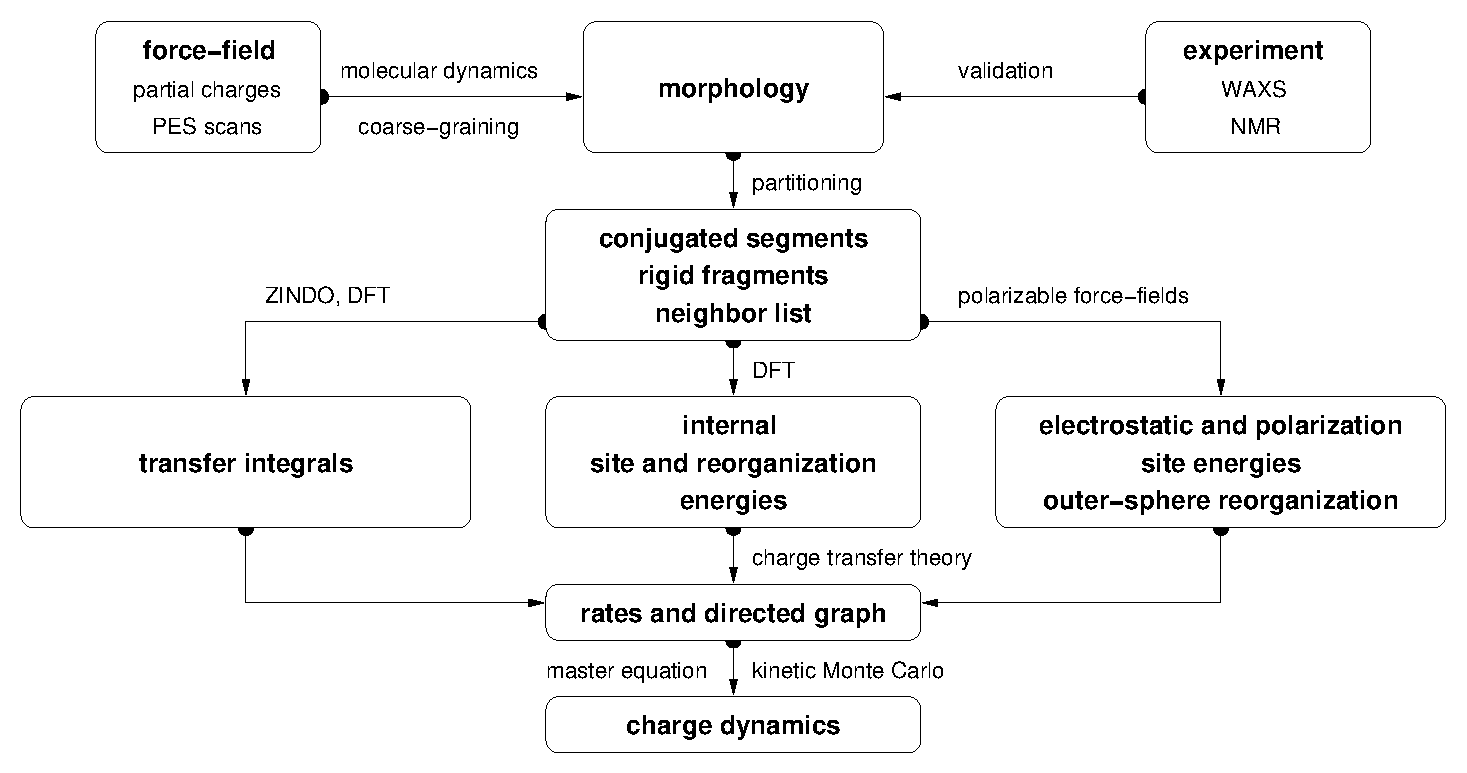
\includegraphics[width=\linewidth]{fig/workflow/workflow}
 \caption{%
   Workflow for microscopic simulations of charge transport.  %
   \label{fig:workflow}}
\end{figure*}

A typical workflow of charge transport simulations is depicted in \fig{workflow}. The first step is the simulation of an \hyperref[sec:morphology]{atomistic morphology}, which is then partitioned on \hyperref[sec:mapping]{hopping sites}. The coordinates of the hopping sites are used to construct a list of pairs of molecules (neighbor list). For each pair an \hyperref[sec:transfer_integrals]{electronic coupling element}, a reorganization energy (sec.~\ref{sec:reorganization}), a driving force (sec.~\ref{sec:edisorder}), and eventually the hopping rate are evaluated. The neighbor list and hopping rates define a directed graph. The corresponding master equation is solved using the kinetic Monte Carlo method (sec.~\ref{sec:me}), which allows to explicitly monitor the charge dynamics in the system as well as to calculate time- or ensemble averages of occupation probabilities, charge fluxes, correlation functions, and field-dependent mobilities (sec.~\ref{sec:analysis}).

The toolkit is implemented using modular concepts introduced earlier in the Versatile Object-oriented Toolkit for Coarse-graining Applications (VOTCA)~\cite{ruehle_versatile_2009}. The VOTCA structures are adapted to reading atomistic trajectories, mapping them onto conjugated segments and rigid fragments, and substituting (if needed) rigid fragments with the optimized copies. 

The \hyperref[sec:moo]{molecular orbital overlap module} calculates electronic coupling elements between  conjugated segments from the corresponding molecular orbitals. It relies on the semi-empirical INDO Hamiltonian and molecular orbitals in the format provided by the \gaussian package. An alternative,  \hyperref[sec:dft]{density-functional based approach}, has interfaces to the \gaussian and \turbomole packages. An interface to the \tinker package is provided for calculations of electrostatic and polarization contributions to energetic disorder. 

The kinetic Monte Carlo module reads in the neighbor list, site coordinates, and hopping rates and performs charge dynamics simulations using either periodic boundary conditions or charge sources and sinks. 

The toolkit is written as a combination of modular C++ code and scripts. The data transfer between programs is implemented via a state file or database, which is also used to restart simulations. Analysis functions and most of the calculation routines are encapsulated by using the observer pattern~\cite{gamma_design_1995} which allows the implementation of new functions as individual modules.